\documentclass[paper=a4, fontsize=11pt]{scrartcl} % A4 paper and 11pt font size

\usepackage[T1]{fontenc} % Use 8-bit encoding that has 256 glyphs
\usepackage{fourier} % Use the Adobe Utopia font for the document - comment this line to return to the LaTeX default
\usepackage[english]{babel} % English language/hyphenation
\usepackage{amsmath,amsfonts,amsthm,amssymb} % Math packages

\usepackage{caption}
\usepackage{graphicx, subfig}

\usepackage{algorithm, algorithmic}
\renewcommand{\algorithmicrequire}{\textbf{Input:}} %Use Input in the format of Algorithm  
\renewcommand{\algorithmicensure}{\textbf{Output:}} %UseOutput in the format of Algorithm  

\usepackage{listings}
\lstset{language=Matlab}

\usepackage{lipsum} % Used for inserting dummy 'Lorem ipsum' text into the template

\usepackage{sectsty} % Allows customizing section commands
\allsectionsfont{\centering \normalfont\scshape} % Make all sections centered, the default font and small caps

\usepackage{fancyhdr} % Custom headers and footers
\pagestyle{fancyplain} % Makes all pages in the document conform to the custom headers and footers
\fancyhead{} % No page header - if you want one, create it in the same way as the footers below
\fancyfoot[L]{} % Empty left footer
\fancyfoot[C]{} % Empty center footer
\fancyfoot[R]{\thepage} % Page numbering for right footer
\renewcommand{\headrulewidth}{0pt} % Remove header underlines
\renewcommand{\footrulewidth}{0pt} % Remove footer underlines
\setlength{\headheight}{13.6pt} % Customize the height of the header

\numberwithin{equation}{section} % Number equations within sections (i.e. 1.1, 1.2, 2.1, 2.2 instead of 1, 2, 3, 4)
\numberwithin{figure}{section} % Number figures within sections (i.e. 1.1, 1.2, 2.1, 2.2 instead of 1, 2, 3, 4)
\numberwithin{table}{section} % Number tables within sections (i.e. 1.1, 1.2, 2.1, 2.2 instead of 1, 2, 3, 4)

\setlength\parindent{0pt} % Removes all indentation from paragraphs - comment this line for an assignment with lots of text

%----------------------------------------------------------------------------------------
%	TITLE SECTION
%----------------------------------------------------------------------------------------

\newcommand{\horrule}[1]{\rule{\linewidth}{#1}} % Create horizontal rule command with 1 argument of height

\title{	
\normalfont \normalsize 
\textsc{Shanghai Jiao Tong University, UM-SJTU JOINT INSTITUTE} \\ [25pt] % Your university, school and/or department name(s)
\horrule{0.5pt} \\[0.4cm] % Thin top horizontal rule
\huge Turbulence \\ HW1 \\ % The assignment title
\horrule{2pt} \\[0.5cm] % Thick bottom horizontal rule
}

\author{Yu Cang \\ 018370210001} % Your name

\date{\normalsize \today} % Today's date or a custom date

\begin{document}

\maketitle % Print the title

\section{Exercise1}
  Let
  \begin{equation}
  	\Phi = \oiiint_\Omega \phi dv
  \end{equation}
  where $\phi$ is the passive scalar, and $\Omega$ is the control volume. \\
  Then the change of $\Phi$ is due to the gradiant diffusion through boundary of $\Omega$, which can be written as
  \begin{equation}
  	\frac{D}{Dt} \Phi = \oiint_{\partial \Omega} \Gamma \nabla \phi d\vec{S}
  \end{equation}
  where $\Gamma$ indicates the diffusivity, with unit of $m^2/s$.\\
  The material derivative of $\Phi$ in Euler field is given as follows using RTT
  \begin{equation}
  	\frac{D}{Dt} \Phi = \oiiint_\Omega \frac{\partial \phi}{\partial t} dv + \oiint_{\partial \Omega} \phi \vec{U} \cdot d\vec{S}
  \end{equation}
  When field of $\phi$ is assumed to be smooth enough, the divergence theorem can be applied, which yields
  \begin{equation}
  	\oiiint_\Omega \frac{\partial \phi}{\partial t} dv + \oiiint_\Omega \nabla \cdot (\phi \vec{U}) dv = \oiiint_\Omega \nabla \cdot (\Gamma \nabla \phi) dv
  \end{equation}
  namely
  \begin{equation}
  	\frac{\partial \phi}{\partial t} + \nabla \cdot (\phi \vec{U}) = \nabla \cdot (\Gamma \nabla \phi)
  \end{equation}
  The equation can be further simplified when the flow is assumed to be both incompressible and constant-property.
  \begin{equation}
  		\frac{\partial \phi}{\partial t} + \vec{U} \cdot \nabla \phi = \Gamma \nabla^2 \phi
  \end{equation}
  which can be written in material derivative format as
  \begin{equation}
  	\frac{D}{Dt}\phi = \Gamma \nabla^2 \phi
  \end{equation}
  
\section{Exercise2}
  Let $X$ and $Y$ be 2 sequences of random numbers, the correlation coefficient of these 2 random variables is calculated as
  \begin{equation}
  	\rho_{XY} = \frac{cov(X, Y)}{\sqrt{E[X^2] E[Y^2]}}
  \end{equation}
  the covariance of $X$ and $Y$ is calculated as
  \begin{equation}
  	cov(X, Y) = E[(X-E[X])(Y-E[Y])] = E[XY] - E[X]E[Y]
  \end{equation}
  With $E[XY], E[X], E[Y], E[X^2], E[Y^2]$ provided, the correlation coefficient can be therefore calculated. And
  numerical experiment has been done with 500 times trial.
   \begin{figure}[H]
	  	\centering
	  	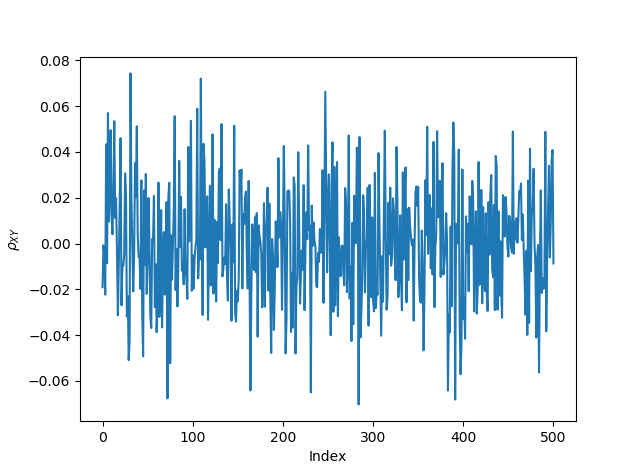
\includegraphics[height=10cm]{CovPlot.png}
	  	\caption{Covariance of random numbers}
	  	\label{img:cov}
  	\end{figure}
\section{Exercise3}

\section{Exercise4}

\end{document}